\documentclass[usenames,dvipsnames]{beamer}
\usepackage{graphicx}
\usepackage{tablefootnote}
\usepackage{bm}
\usepackage{amsmath}
\usepackage{array, booktabs, multicol,hyperref}
\usepackage{ulem}


% Algorithms package
\usepackage[vlined, ruled, lines numbered]{algorithm2e}

% Tikz
\usepackage{tikz}
\usetikzlibrary{shapes}

\usepackage{url}

% LaTeX commands added by CCKM to process tables
% Adjust separation between rows
\renewcommand{\arraystretch}{1.1}
% Commands which allow the width to be set
\newcolumntype{L}[1]{>{\raggedright \let\newline\\\arraybackslash\hspace{0pt}}m{#1}}
\newcolumntype{C}[1]{>{\centering   \let\newline\\\arraybackslash\hspace{0pt}}m{#1}}
\newcolumntype{R}[1]{>{\raggedleft  \let\newline\\\arraybackslash\hspace{0pt}}m{#1}}

% Augmented vector notation
\newcommand{\av}[2]{\langle #1, #2 \rangle}



\graphicspath{{../fig/}{../../report/fig/}}

\beamertemplatenavigationsymbolsempty

\setbeamertemplate{footline}[frame number]
\definecolor{bostonuniversityred}{rgb}{0.8, 0.0, 0.0}
\usetheme{Copenhagen}

\title[Accuracy and smoothness]{The need for accuracy and smoothness in numerical simulations}

\author[Carl Christian Kjelgaard Mikkelsen et al.]{\underline{Carl Christian Kjelgaard Mikkelsen} \and
Lori{\'e}n L{\'o}pez-Villellas}

\institute{
  Department of Computer Science, Ume{\aa} University, Sweden, \\ {\tt spock@cs.umu.se} \and Department of Computer Science, Zaragoza University, Spain, \\ {\tt lorien.lopez@unizar.es}
}


\date{Visit to FSHMN \\ Pristina, Kosovo, September 12th 2024}


\titlegraphic{
  \vspace*{0mm}
  \centering
  
\includegraphics[height=1.0cm]{umu-logotyp-EN.png} \;\;
  
\includegraphics[height=1.5cm]{Solemne_color.png} \;\;
  
\includegraphics[height=1.0cm]{87660_essence_rgb.png}
}

\begin{document}

\frame{\titlepage} 

\frame{\frametitle{Introduction}

  \begin{itemize}
  \item Danish nationality
  \item Ass. Prof. of Comp. Sci. at Ume{\aa} University, Sweden
  \item Ph.D in mathematics from Purdue University, Indiana, USA
  \item MSc. in mathematics from Aarhus University, Denmark
  \item Research interests
    \begin{itemize}
    \item Structured linear system
    \item Nonsymmetric eigenvalue problems
    \item Solution of nonlinear constraint equations
    \item High performance scientific computing
    \end{itemize}
  \item Software
    \begin{itemize}
    \item Coauthor of StarNEIG
    \item Coauthor of ILVES
    \end{itemize}
  \end{itemize}
}

%% \frame{\frametitle{A simple experiment}

%%   We did two sets of simulations of a molecule in water
%%   \vspace{1cm}
%%   \begin{enumerate} \setlength\itemsep{1em}
%%     \item fixed real time
%%     \item two different force-fields: \texttt{charmm36}, \texttt{oopsaal}
%%     \item identical initial conditions
%%     \item ran the constraint solver to stagnation
%%    \end{enumerate}
%%   \vspace{1cm}
%%   and tracked the final energy as a function of the number of steps.

%% }

%% \frame{% \frametitle{Warning: Disturbing pictures below}

%%  \begin{figure}
%%     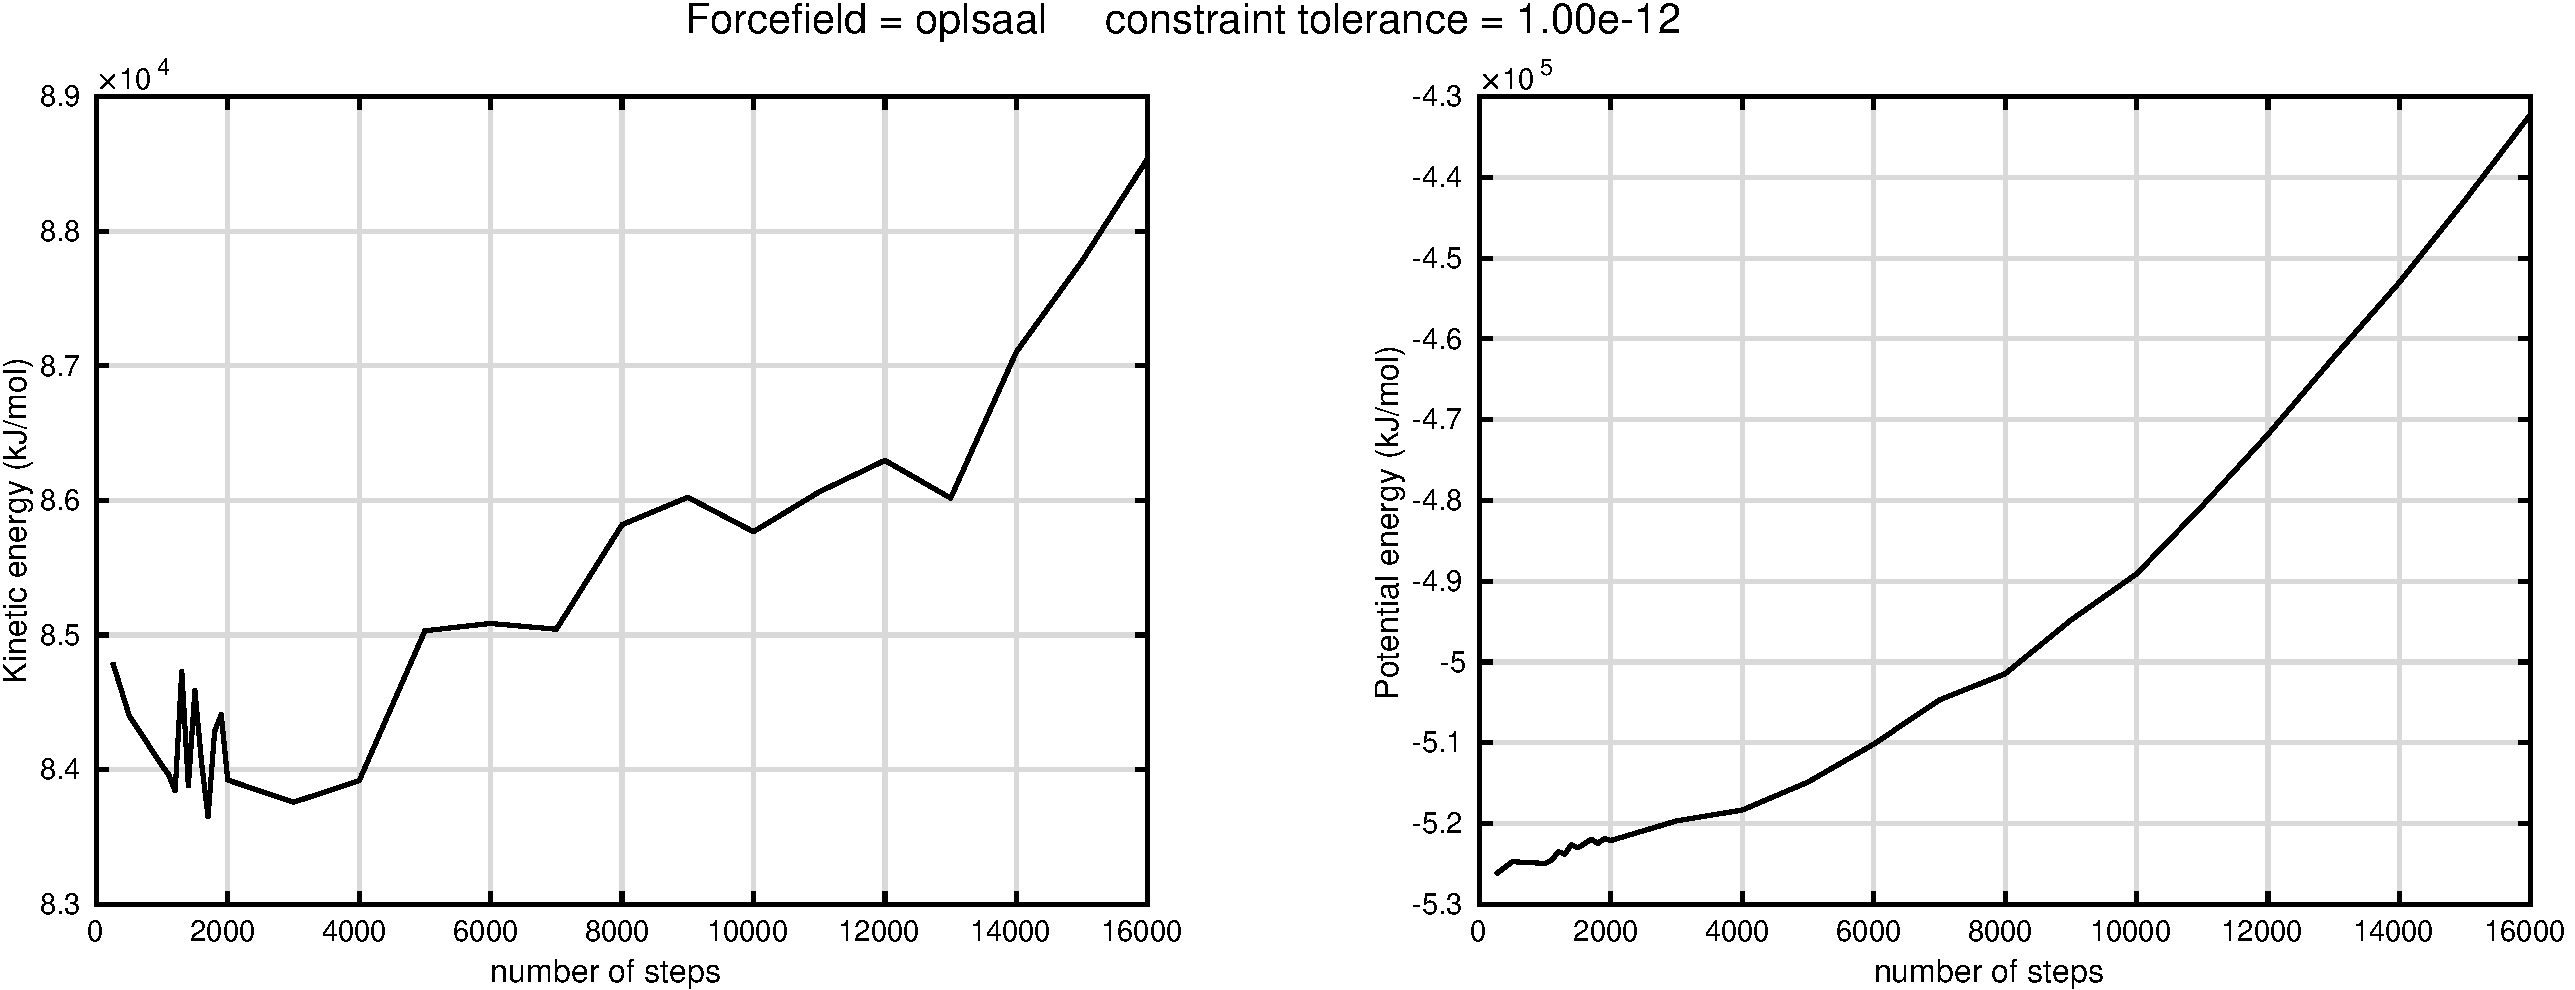
\includegraphics[width=10.5cm]{oplsaaltol12.pdf}
%%   \end{figure}

%%   \begin{figure}
%%     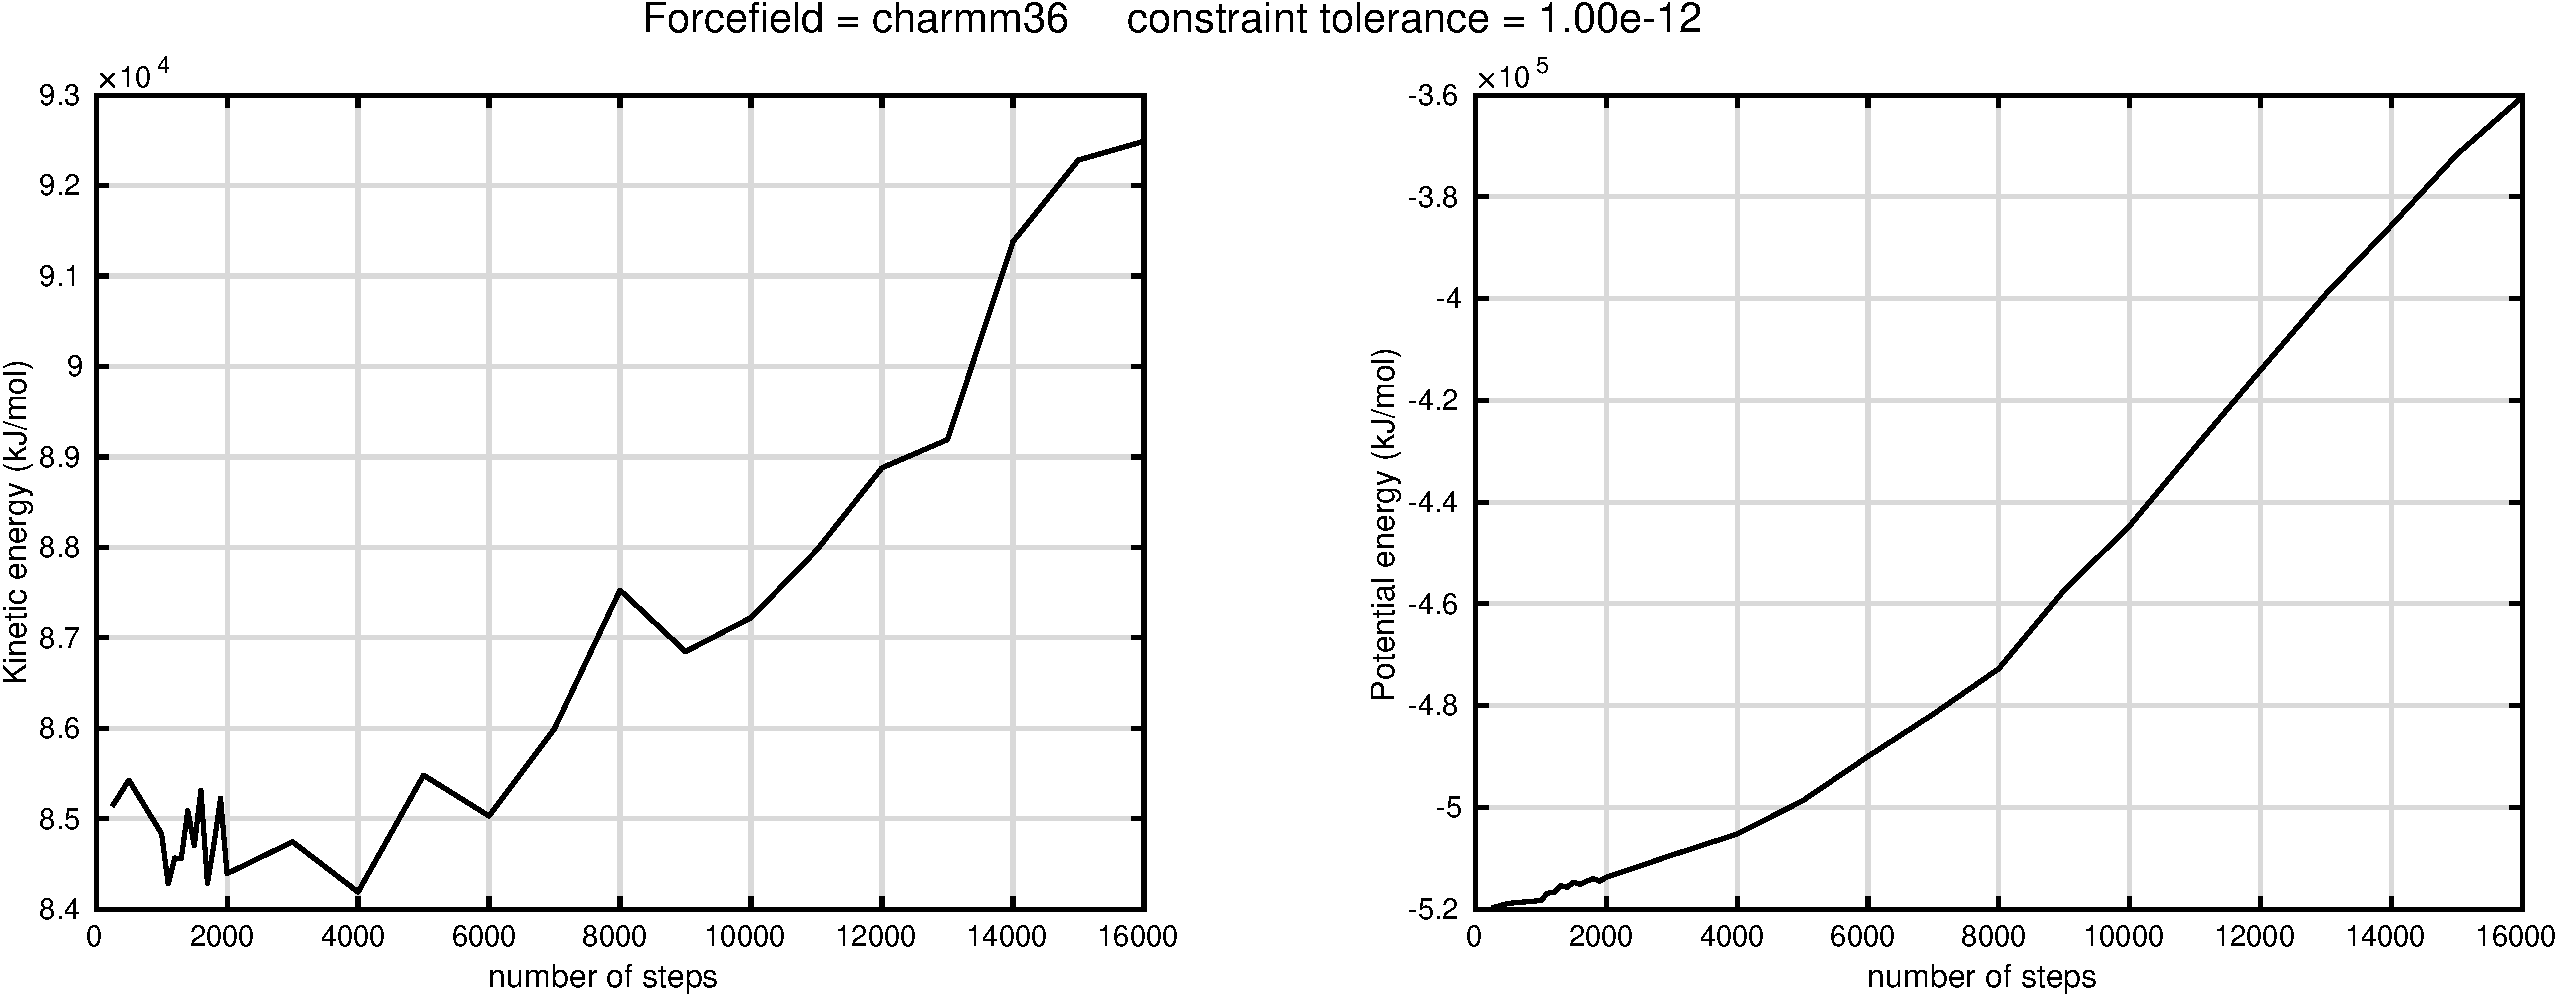
\includegraphics[width=10.5cm]{charmm36tol12.pdf}
%%   \end{figure}

%% }




\frame{\frametitle{External ballistics}

  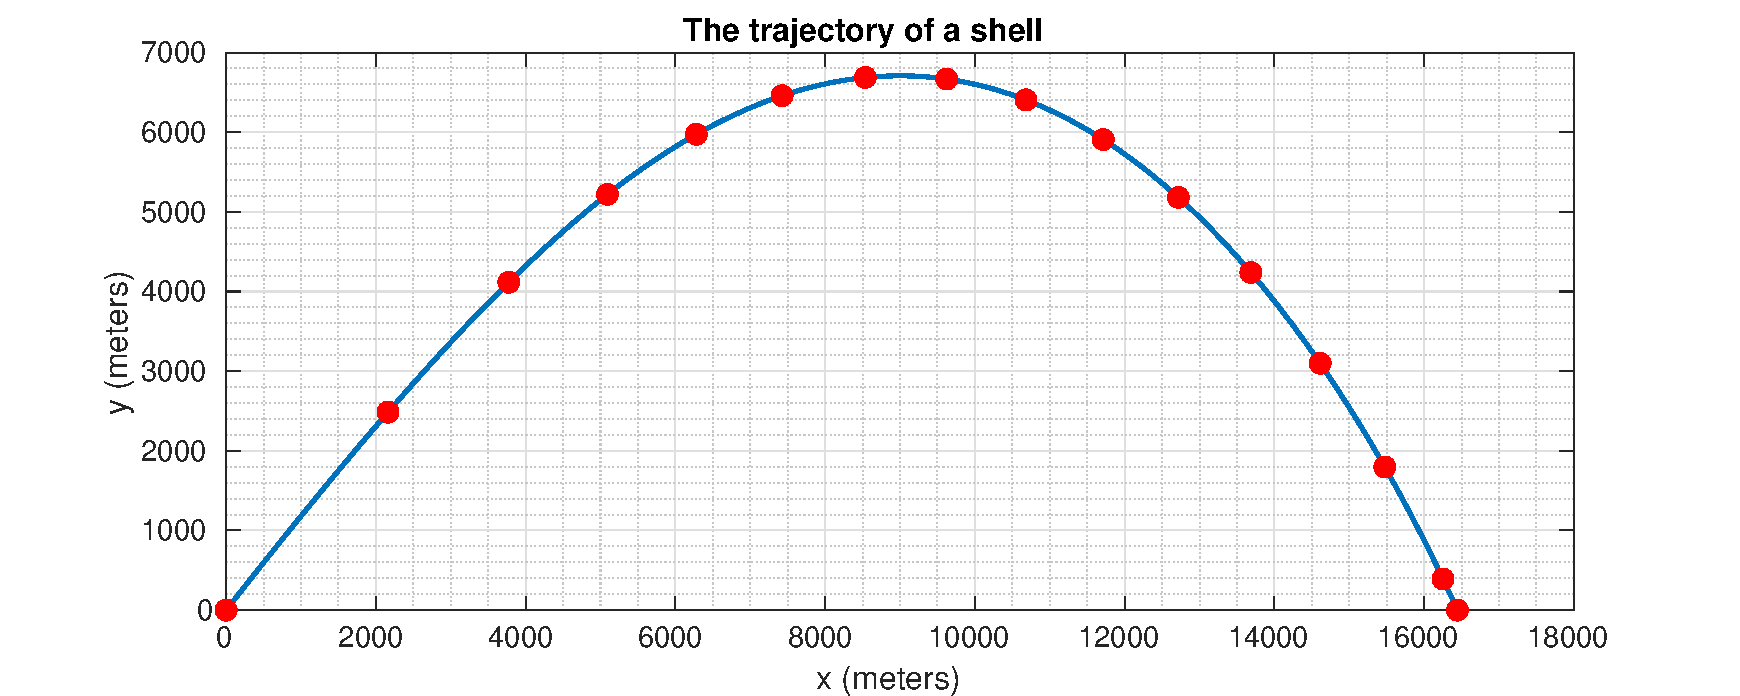
\includegraphics[width=12cm]{range_rk1_mwe2.pdf}

  The total force $\bm{F}$ acting on the shell 
  \begin{equation}
    \bm{F} = m \bm{g} - \frac{1}{2} \rho(y) A C_D(\nu) \|\bm{v} - \bm{w}\|_2 ( \bm{v} - \bm{w} )
  \end{equation}
  is the combination of gravity and aerodynamic drag.
}


\frame{\frametitle{External ballistics}

\begin{block}{Key questions}
  Does it matter
  \begin{enumerate}
  \item if the drag coefficient
    \begin{equation*}
      \nu \rightarrow C_D(\nu)
    \end{equation*}
    is smooth or not?
  \item if the event equation
    \begin{equation*}
      y(t) = 0
    \end{equation*}
    is solved accurately or not?
      \end{enumerate}
 \end{block}
}


\frame{\frametitle{Molecular dynamics with constraints}

  The system of differential algebraic equations
  \begin{align}
  \bm{q}'(t) &= \bm{v}(t), \\
  \bm{M}\bm{v}'(t) &= \bm{f}(\bm{q}(t)) - \bm{G}(\bm{q}(t))^T\bm{\lambda}(t), \\
  \bm{g}(\bm{q}(t)) &= \bm{0}. 
  \end{align}
  is solved using the SHAKE algorithm
  \begin{align}
  \bm{v}_{n+1/2} &= \bm{v}_{n-1/2} + \bm{h} \bm{M}^{-1} \left( \bm{f}(\bm{q}_n) - \bm{G}(\bm{q}_n)^T \bm{\lambda} \right), \\
  \bm{q}_{n+1} &= \bm{q}_n + h \bm{v}_{n + 1/2}, \\
  \bm{g}(\bm{q}_{n+1}) &= \bm{0}. \label{equ:constraint}
\end{align}
}

\frame{\frametitle{Molecular dynamics}

  \begin{block}{Key questions}
    Does it matter\vspace{0.5cm}
    \begin{enumerate}\setlength\itemsep{1.5em}
    \item if the force-field 
      \begin{equation*}
        \bm{q} \rightarrow \bm{f}(\bm{q})
      \end{equation*}
      is smooth or not?
    \item if the nonlinear constraint equation
      \begin{equation*}
        \bm{g}(\bm{q}_{n+1}(\bm{\lambda})) = \bm{0}
      \end{equation*}
      is solved accurately with respect to $\bm{\lambda}$ or not?
    \end{enumerate}
  \end{block}
}


\frame{\frametitle{The primary point of this talk}
  
  If one of the following is true:
  \vspace{0.5cm}
  \begin{enumerate}
  \item the central functions are not smooth enough
  \item the central equations are not solved accurately enough
  \end{enumerate}
  \vspace{0.5cm}
  then we will almost certainly lose the ability to
  \vspace{0.5cm}
  \begin{enumerate}
  \item assert that \underline{rounding} errors are irrelevant
  \item estimate the \underline{discretization} error
  \item estimate the \underline{modelling} error
  \end{enumerate}
  \vspace{1cm}
}


\frame{\frametitle{The key terms of this talk}

  \begin{enumerate} \setlength\itemsep{1em}
  \item $P$: physical quantity that can be measured
  \item $T$: approximation of $P$ predicted by our model 
  \item $A_h$: approximation of $T$ returned by our algorithm
  \item $\hat{A}_h$: the computed value of $A_h$.
  \end{enumerate}
}


\frame{\frametitle{The three different error terms}

  \begin{enumerate}
  \item $P - T$ is the modelling error and
    \begin{equation}
      P - T \not = 0
    \end{equation}
    because our model is simpler than the real world.
  \item $T - A_h$ is the discretization error and
    \begin{equation}
      T - A_h \not = 0
    \end{equation}
    because we cannot solve most differential equations exactly.
  \item $A_h - \hat{A}_h$ is the computational error and
    \begin{equation}
      A_h - \hat{A}_h \not = 0
    \end{equation}
    due to rounding errors and truncation errors.
  \end{enumerate}
}

\frame{\frametitle{Why should we care?}

  We validate our models by demonstrating that
  \begin{equation}
    P - T \approx 0
  \end{equation}
  is a good approximation, but
  \begin{equation}
    P - T \approx P - \hat{A}_h
  \end{equation}
  is not necessarily a good approximation. We have
  \begin{equation}
    \underset{\text{modelling error}}{\underbrace{P - T}} = (P - \hat{A}_h) - \underset{\text{discretization error}}{\underbrace{(T - A_h)}} - \underset{\text{computational error}}{\underbrace{(A_h - \hat{A}_h)}}
  \end{equation}
  so we need to assert that
  \begin{align}
     |T- A_h| & \ll |P - \hat{A}_h| \\
     |A_h - \hat{A}_h| & \ll |P - \hat{A}_h|
  \end{align}
}

\frame{\frametitle{Practical error estimation}

  It is frequently possible to simultanously
   \vspace{0.5cm}
  \begin{enumerate} \setlength\itemsep{1.5em}
  \item assert that the computational error
    \begin{equation*}
      A_h - \hat{A}_h
    \end{equation*}
    is irrelevant, and
  \item estimate the discretization error
    \begin{equation*}
      T_h - A_h
    \end{equation*}
    accurately
  \end{enumerate}
}

\frame{\frametitle{Practical error estimation}

 
  The key is to have an asymptotic error expansion (AEX)
  \begin{equation}
    E_h = T - A_h = \alpha h^p + \beta h^q + O(h^r), \quad h \rightarrow 0_+
  \end{equation}
  where
  \begin{equation}
    0 < p < q < r
  \end{equation}
  are not necessarily integers and $\alpha$, $\beta$ are independent of $h$.
}


\frame{\frametitle{Basic definitions}

We define Richardson's error estimate by
\begin{equation}
  R_h := \frac{A_h - A_{2h}}{2^p - 1}
\end{equation}
and Richardson's fraction by
\begin{equation}
\quad F_h:= \frac{A_{2h} - A_{4h}}{A_h - A_{2h}} 
\end{equation}
}

\frame{\frametitle{Elementary results}
  If
 \begin{equation}
    E_h = T - A_h = \alpha h^p + \beta h^q + O(h^r), \quad h \rightarrow 0_+
  \end{equation}
 then
 \begin{equation}
  \frac{E_h - R_h}{h^q} \rightarrow \text{constant}
\end{equation}
 and
\begin{equation}
  \frac{2^p - F_h}{h^{q-p}} \rightarrow \text{constant}
\end{equation}
}

\frame{\frametitle{Implications}

  \begin{enumerate}
  \item We can determine $p$ from
    \begin{equation}
      F_h \rightarrow 2^p
    \end{equation}
  \item We can determine $q$ from
    \begin{equation}
      \log | 2^p - F_h| \approx \log|\text{constant}| + (q-p) \log h
    \end{equation}
  \item We can then compute $R_h$ and estimate
    \begin{equation}
      E_h \approx R_h
    \end{equation}
    when $h$ is \textit{sufficiently} small.
  \end{enumerate}
}

\frame{\frametitle{Numerical integration \texttt{rint\_mwe1}}

  Our target value is 
  \begin{equation}
    T = \int_0^1 f(x) dx, \quad f(x) = \exp(x)
  \end{equation}
  Our approximation is the composite trapezoidal rule
  \begin{equation}
    A_h = \frac{h}{2} \sum_{j=0}^{n-1} \left( f(x_i) + f(x_{i+1}) \right), \quad x_i = ih, \quad nh = 1
  \end{equation}
  We compute $A_h$ for
  \begin{equation}
    h = h_k = 2^{-k}
  \end{equation}
}


\frame{\frametitle{The evolution of $F_h$ and the quality of $R_h$}

  \begin{figure}[ht]
        \begin{minipage}[b]{0.45\linewidth}
            \centering
            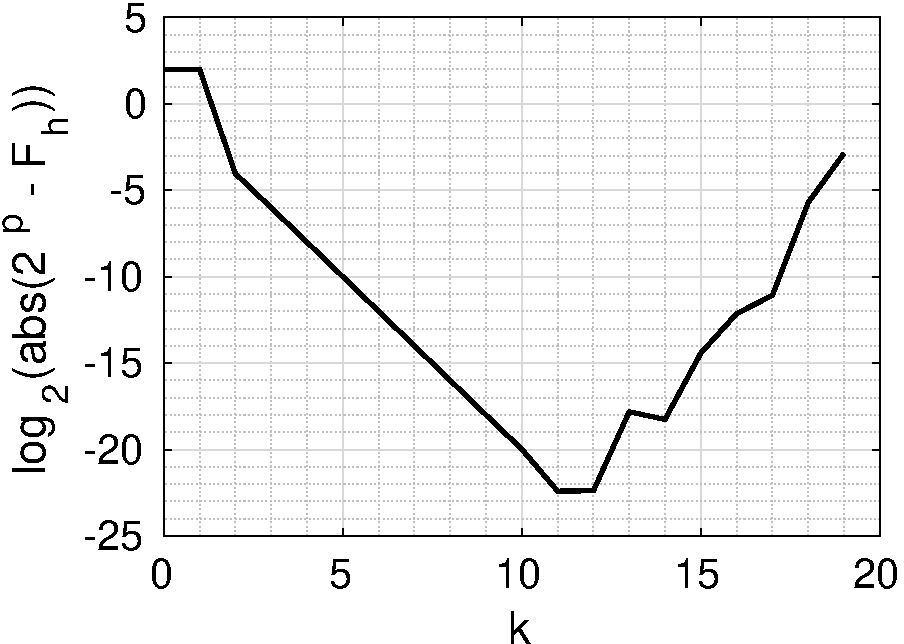
\includegraphics[width=\textwidth]{rint_mwe1a.pdf}
            \caption{The evolution of $F_h$}
            \label{fig:a}
        \end{minipage}
        \hspace{0.5cm}
        \begin{minipage}[b]{0.45\linewidth}
            \centering
            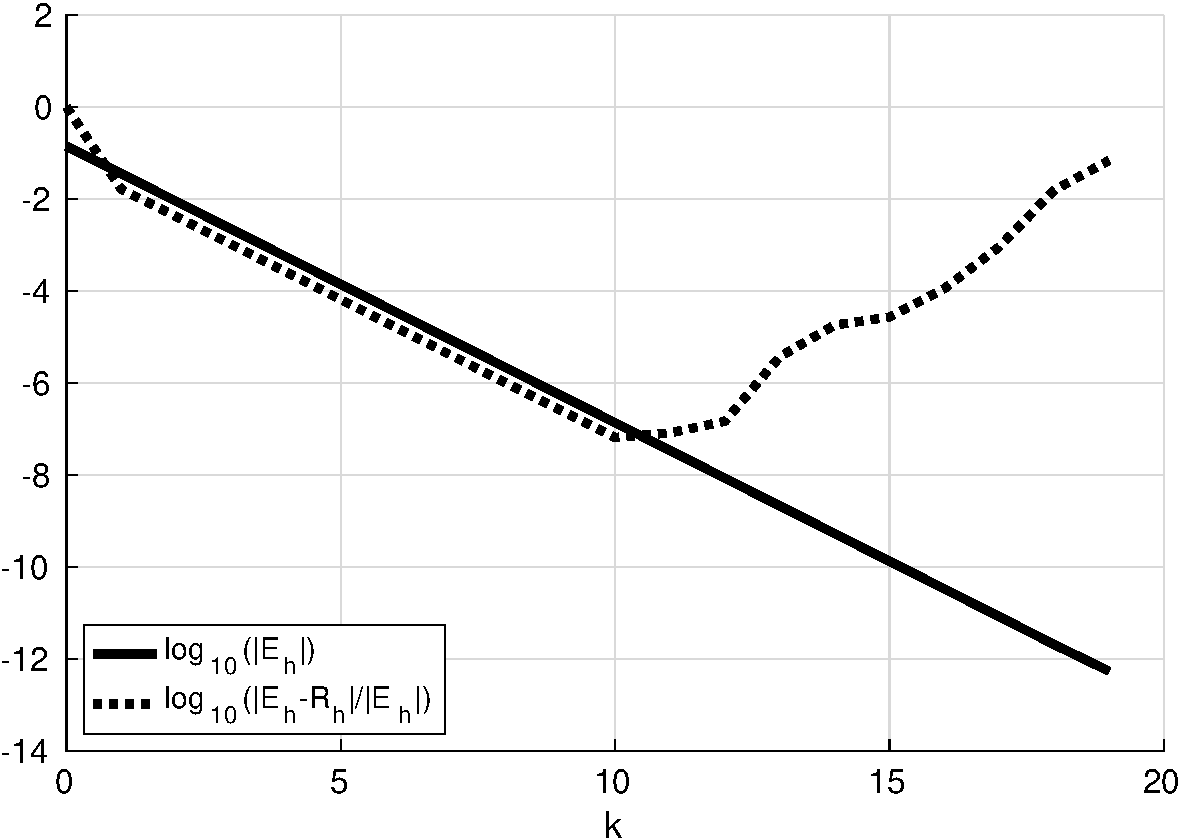
\includegraphics[width=\textwidth]{rint_mwe1b.pdf}
            \caption{The accuracy of $R_h$}
            \label{fig:b}
        \end{minipage}
    \end{figure}
    Strictly speaking we are not observing $F_h$ and $R_h$
  \begin{center}
    we are observing $\hat{F}_h$ and $\hat{R}_h$
  \end{center}
  The difference is controlled by the computational error
  \begin{equation}
    A_h - \hat{A}_h
  \end{equation}
}



\frame{\frametitle{Numerical integration \texttt{rint\_mwe2}}

  Our target value is 
  \begin{equation}
    T = \int_0^1 f(x) dx, \quad f(x) = \sqrt{x}.
  \end{equation}
  Our approximation is the composite trapezoidal rule
  \begin{equation}
    A_h = \frac{h}{2} \sum_{j=0}^{n-1} \left( f(x_i) + f(x_{i+1}) \right), \quad x_i = ih, \quad nh = 1
  \end{equation}
  We compute $A_h$ for
  \begin{equation}
    h = h_k = 2^{-k}
  \end{equation}
}


\frame{\frametitle{The evolution of $F_h$ and the quality of $R_h$}

  \begin{figure}[ht]
        \begin{minipage}[b]{0.45\linewidth}
            \centering
            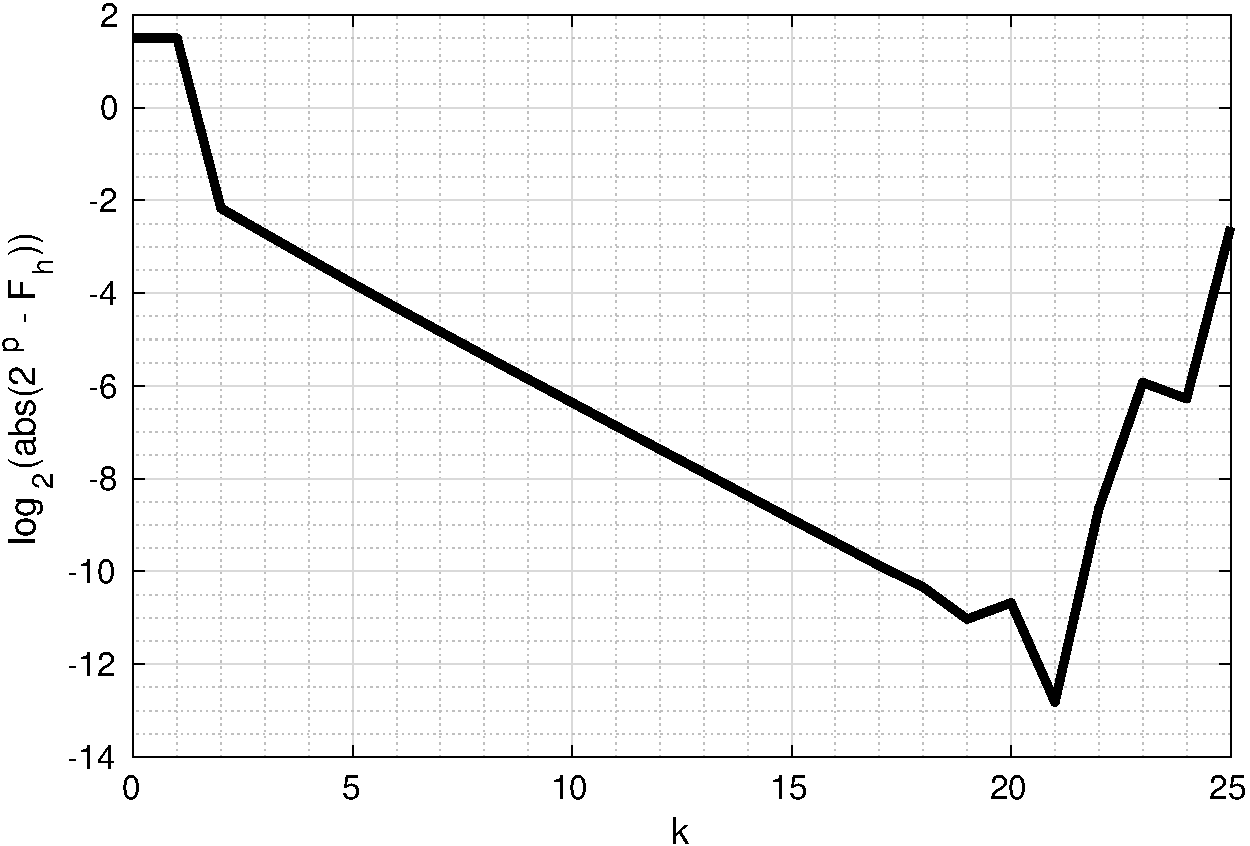
\includegraphics[width=\textwidth]{rint_mwe2a.pdf}
            \caption{The evolution of $F_h$}
            \label{fig:a}
        \end{minipage}
        \hspace{0.5cm}
        \begin{minipage}[b]{0.45\linewidth}
            \centering
            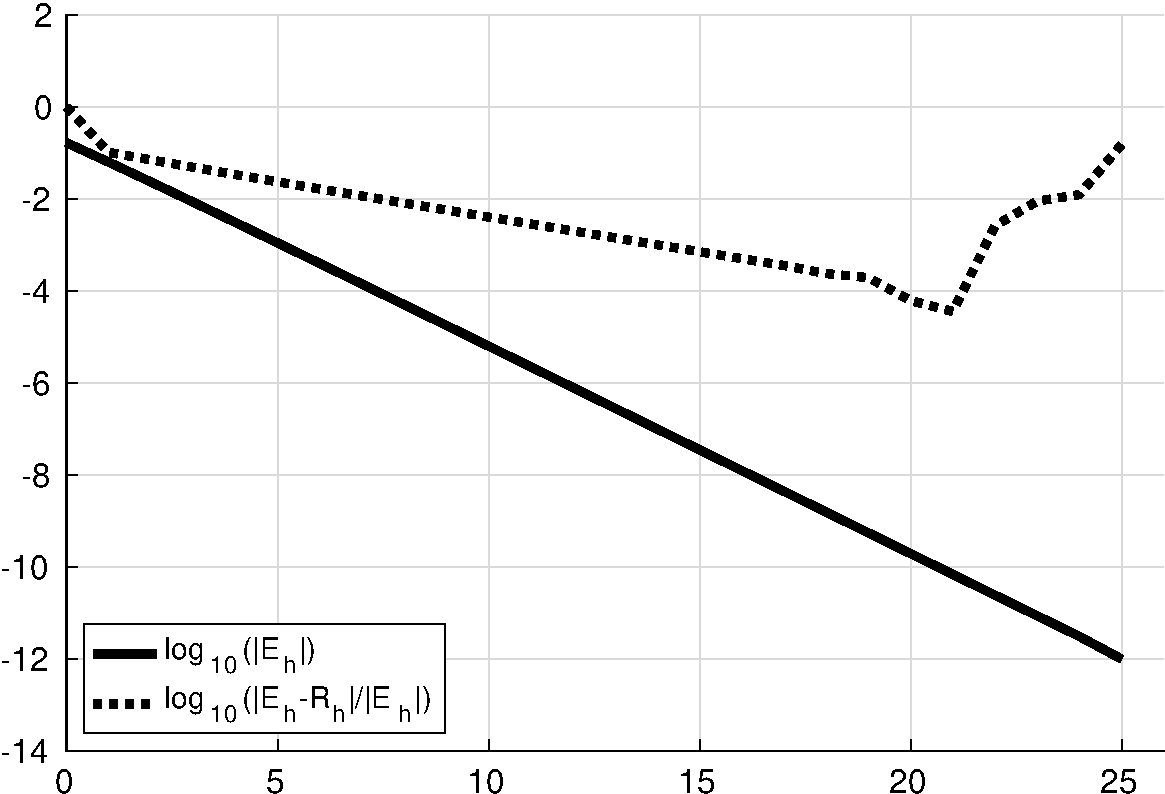
\includegraphics[width=\textwidth]{rint_mwe2b.pdf}
            \caption{The accuracy of $R_h$}
            \label{fig:b}
        \end{minipage}
    \end{figure}
  We observe that
  \begin{enumerate}
  \item the asymptotic range is much wider (good!)
  \item the error estimate is less accurate (mostly harmless)
  \end{enumerate}
  
}






\frame{\frametitle{A spectacular failure}

  GROMACS simulation of hen egg white lysozyme in water:
  \vspace{0.25cm}
  \begin{enumerate} \setlength\itemsep{1em}
  \item $T$: total energy of the simulation at the end
  \item $A_h$: the approximation of $T$ computed using SHAKE
  \item $\hat{A}_h$: the value of $A_h$ returned by the computer
  \end{enumerate}
\vspace{0.5cm}
Temporal matters:
\vspace{0.25cm}
  \begin{enumerate}
  \item The length of the simulations was $10^{-12}$ s ($1$ ps)
  \item A common step size in MD is $10^{-15} s$ ($1$ fs) or $n=1000$ steps
  \item $n \in \{250,500,1000:100:2000,3000:1000:16000\}$
  \end{enumerate}
  
  \begin{center}
   What could possibly go wrong?
  \end{center}
}

\frame{\frametitle{A spectacular failure}

  \begin{figure}
    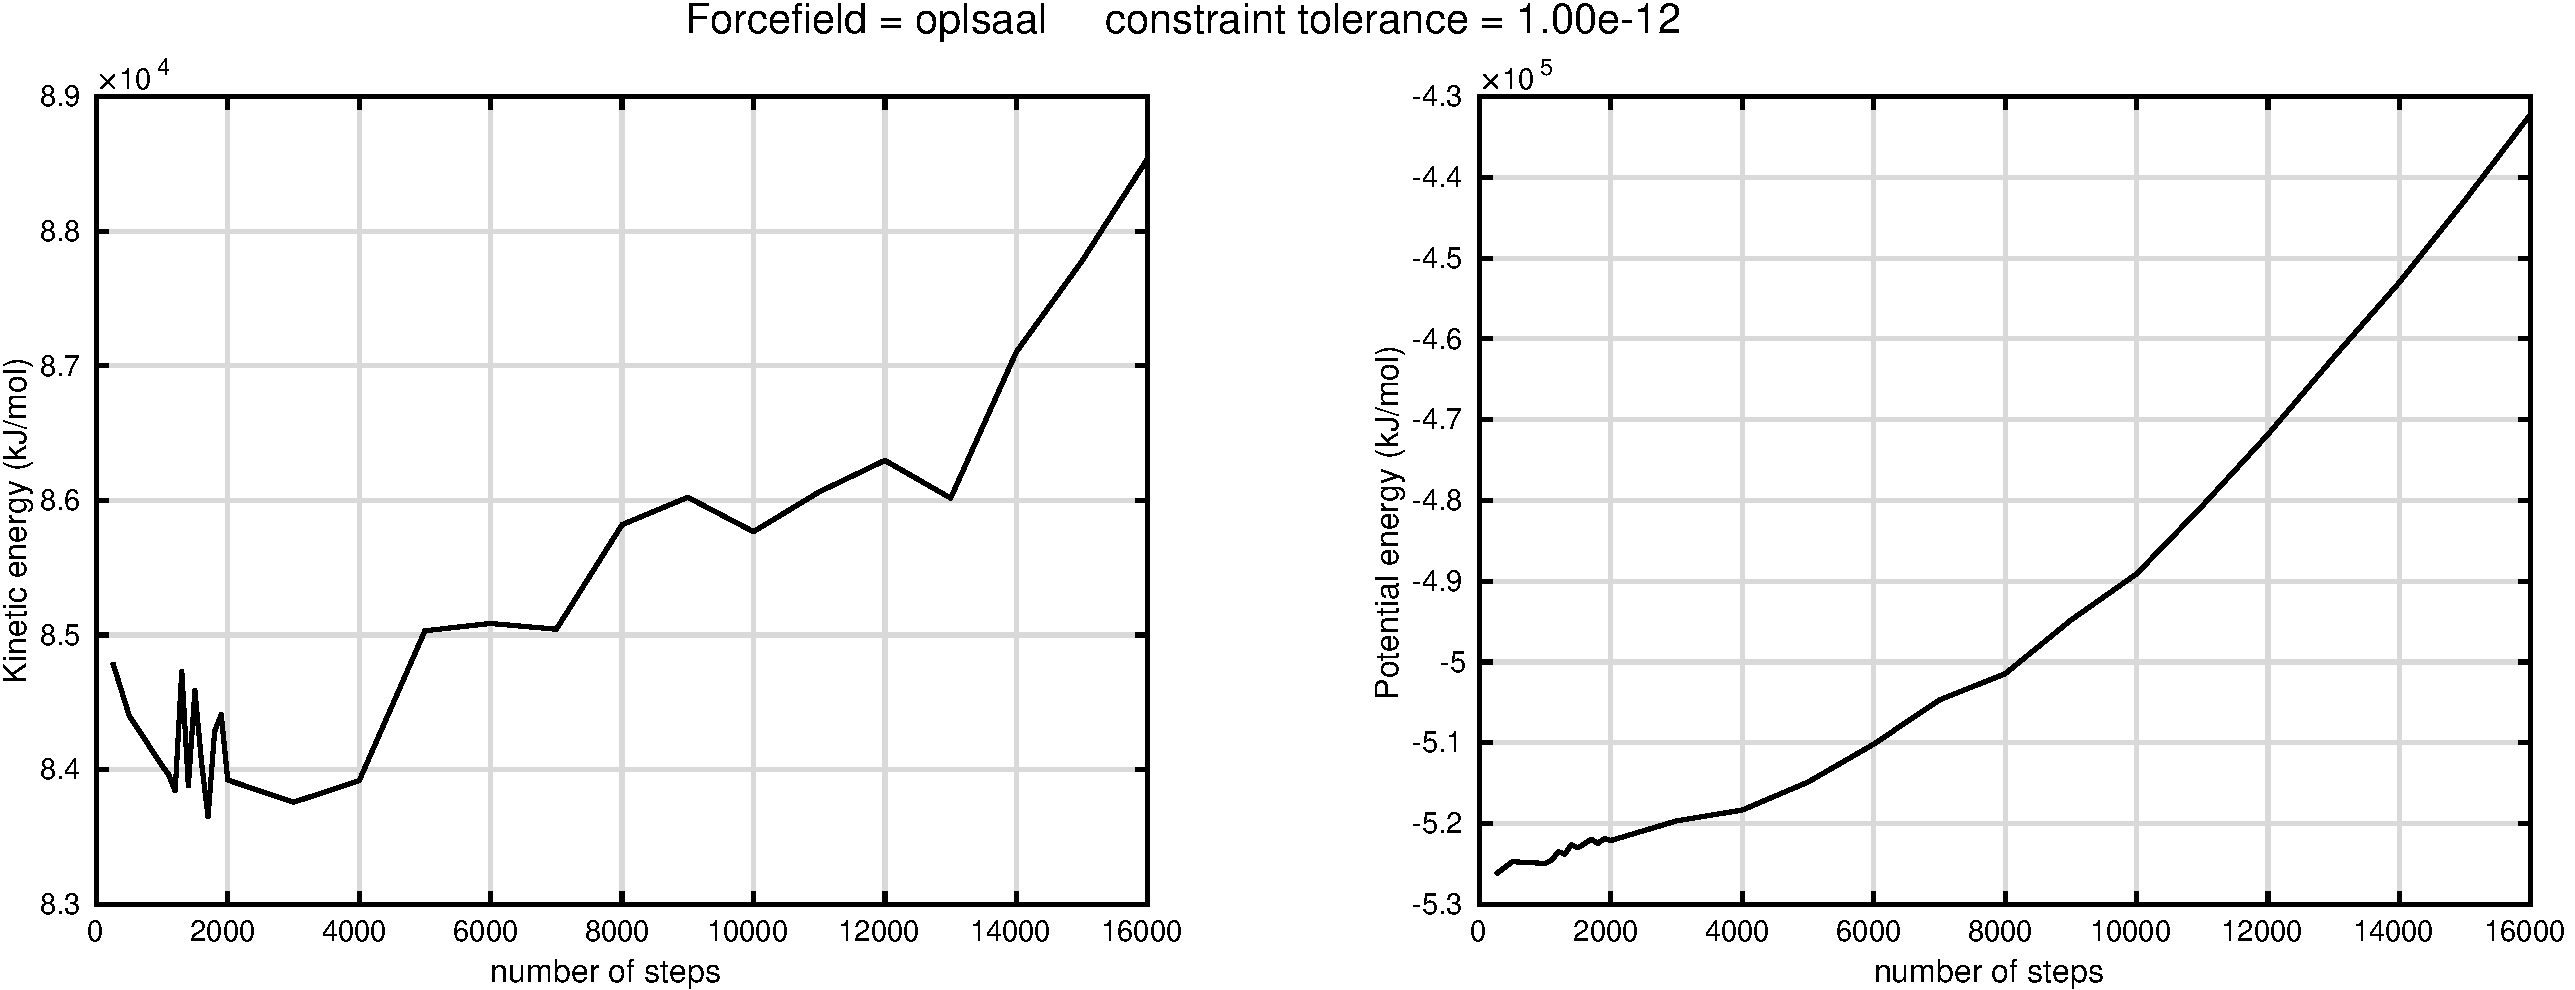
\includegraphics[width=10cm]{oplsaaltol12.pdf}
  \end{figure}
   The rapid growth of the energy for large value of $n$ 
    \begin{center}
      can likely be cured using compensated summation.
    \end{center}
  }

\frame{\frametitle{A spectacular failure}

  \begin{figure}
    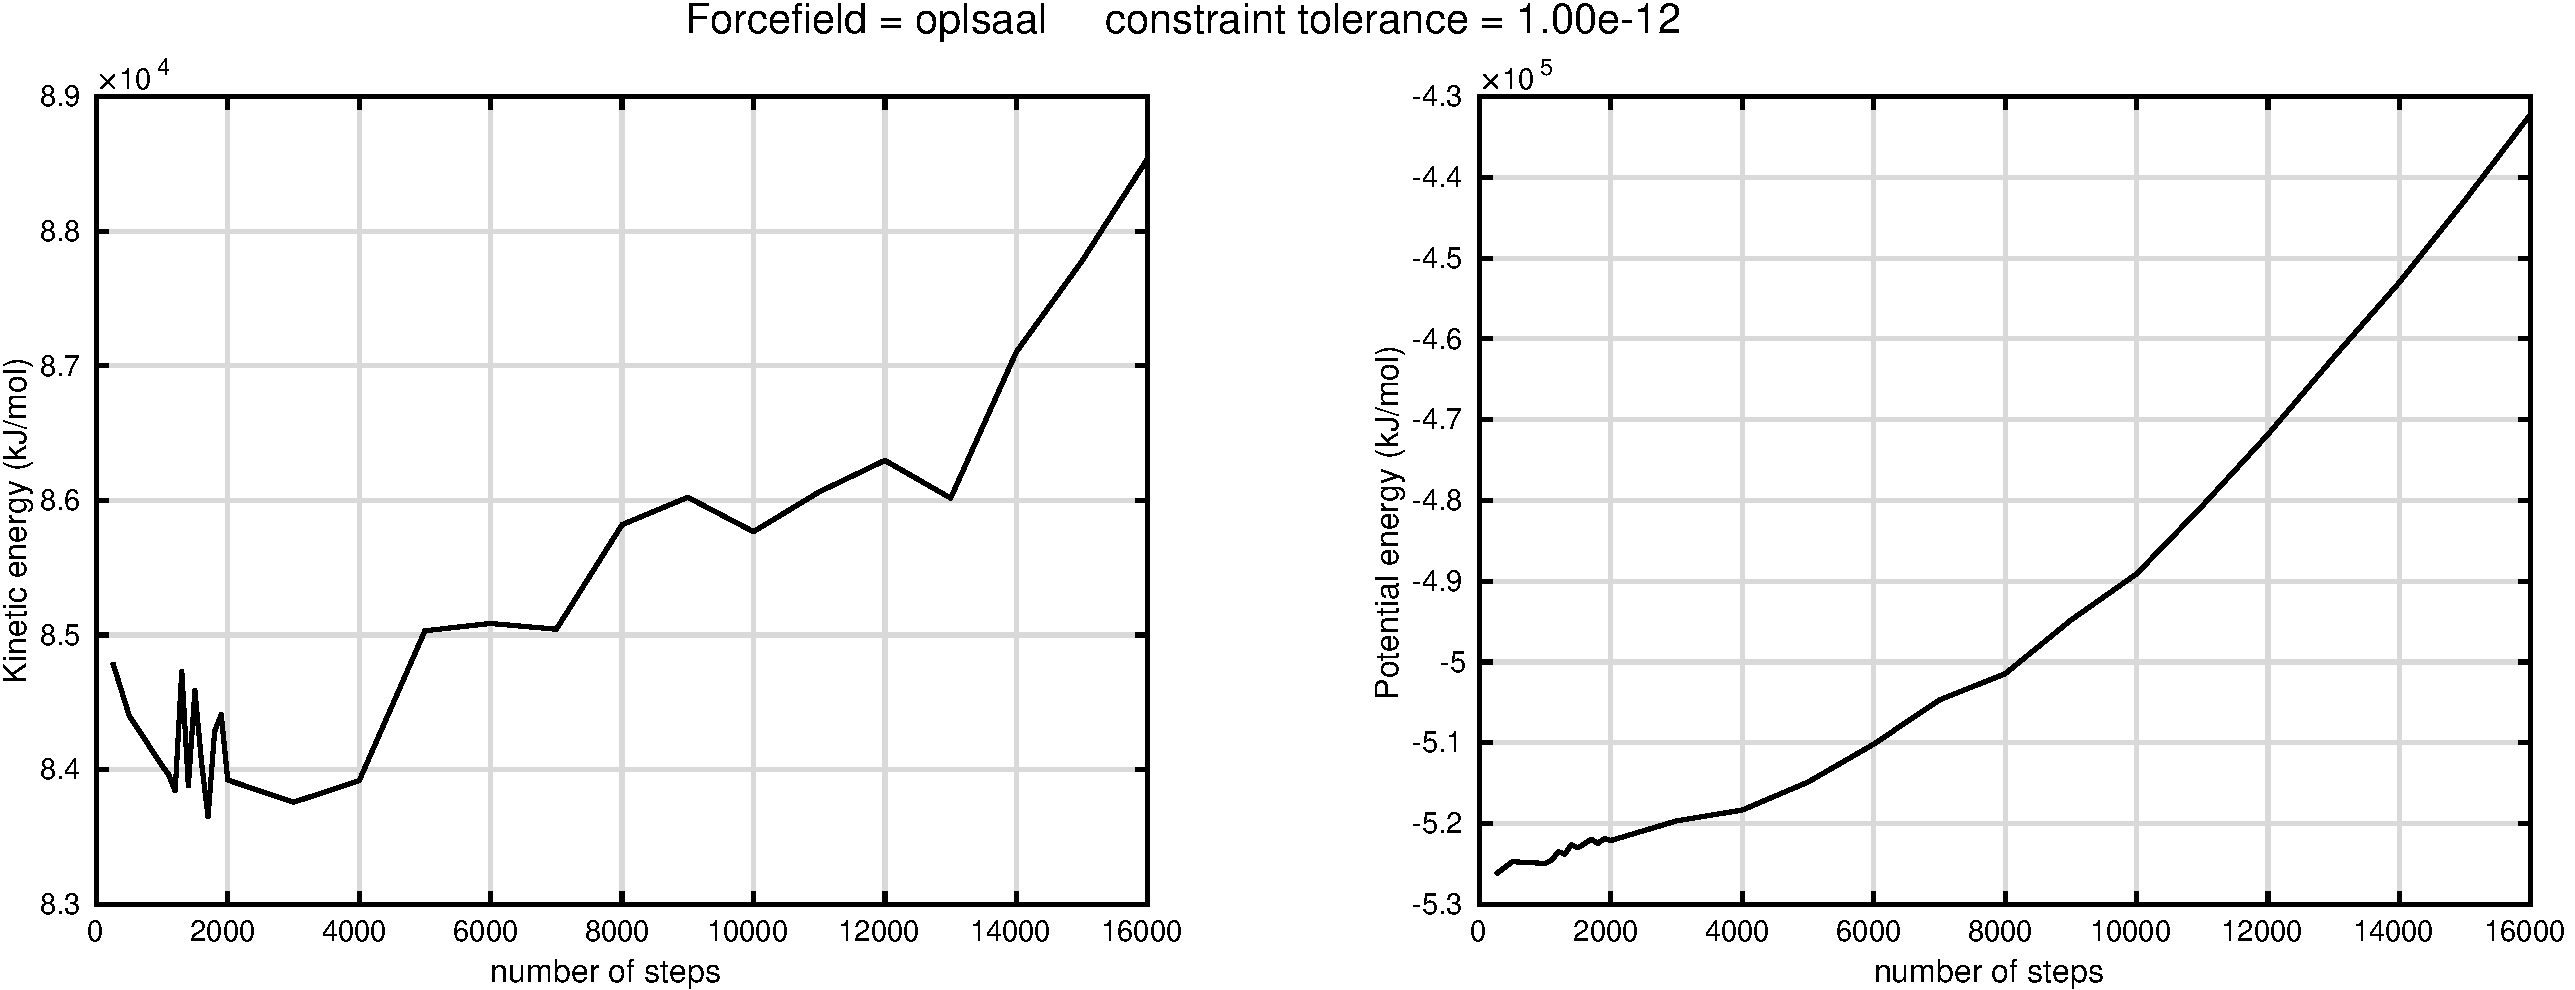
\includegraphics[width=11cm]{oplsaaltol12.pdf}
  \end{figure}
  
  \begin{itemize}
  \item The \underline{wiggles} near $n=1000$ steps are a great concern.
  \item If there is an AEX, then $1$ fs is \underline{not} inside the asymp. range.
  \item We cannot assert that rounding errors are irrelevant
  \item We cannot estimate the discretication error
  \end{itemize}

}


\frame{\frametitle{When do we have an AEX?}

  \begin{enumerate} \setlength\itemsep{1.5em}
  \item Every AEX refers to the exact value of the $A_h$. If
    $$\hat{A}_h \approx A_h$$
    is not a good approximation, then
    \vspace{0.25cm}
    \begin{center}
      $\hat{A}_h$ will not behave nicely
    \end{center}
    \vspace{0.25cm}
    and we cannot identify the asymptotic range.
  \item Deriving an AEX is an exercise in Taylor expansions. If
    \vspace{0.25cm}
    \begin{center}
      our functions are not many times differentiable
    \end{center}
    \vspace{0.25cm}
    then the foundation crumbles.
  \end{enumerate}
}


\frame{\frametitle{External ballistics}

  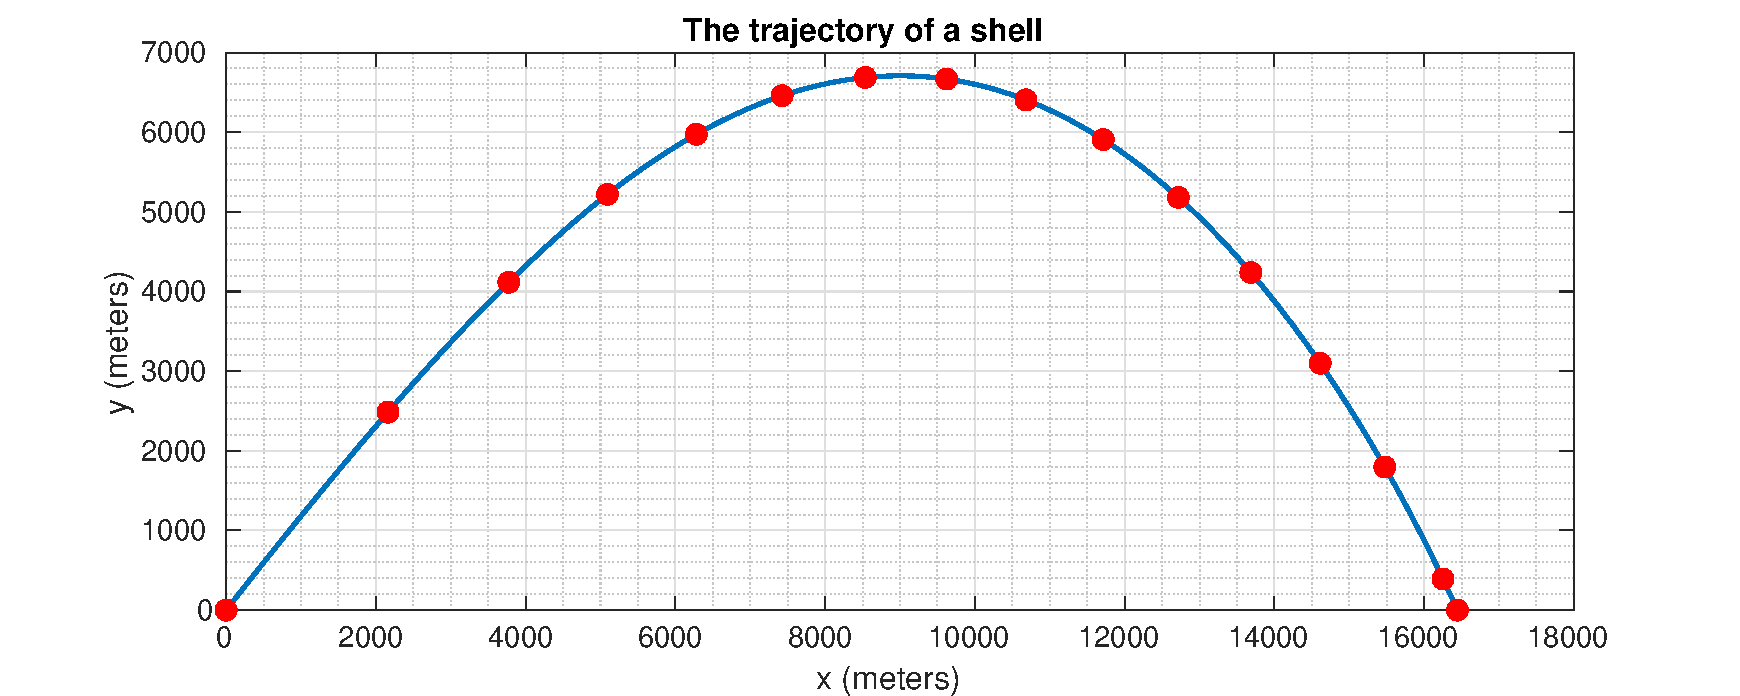
\includegraphics[width=12cm]{range_rk1_mwe2.pdf}

  The total force $\bm{F}$ acting on the shell 
  \begin{equation}
    \bm{F} = m \bm{g} - \frac{1}{2} \rho(y) A C_D(\nu,y) \|\bm{v} - \bm{w}\|_2 ( \bm{v} - \bm{w} )
  \end{equation}
  is the combination of gravity and aerodynamic drag.
}


\frame{\frametitle{Computing the optimal range of the a howitzer: Success}

 \begin{figure}
    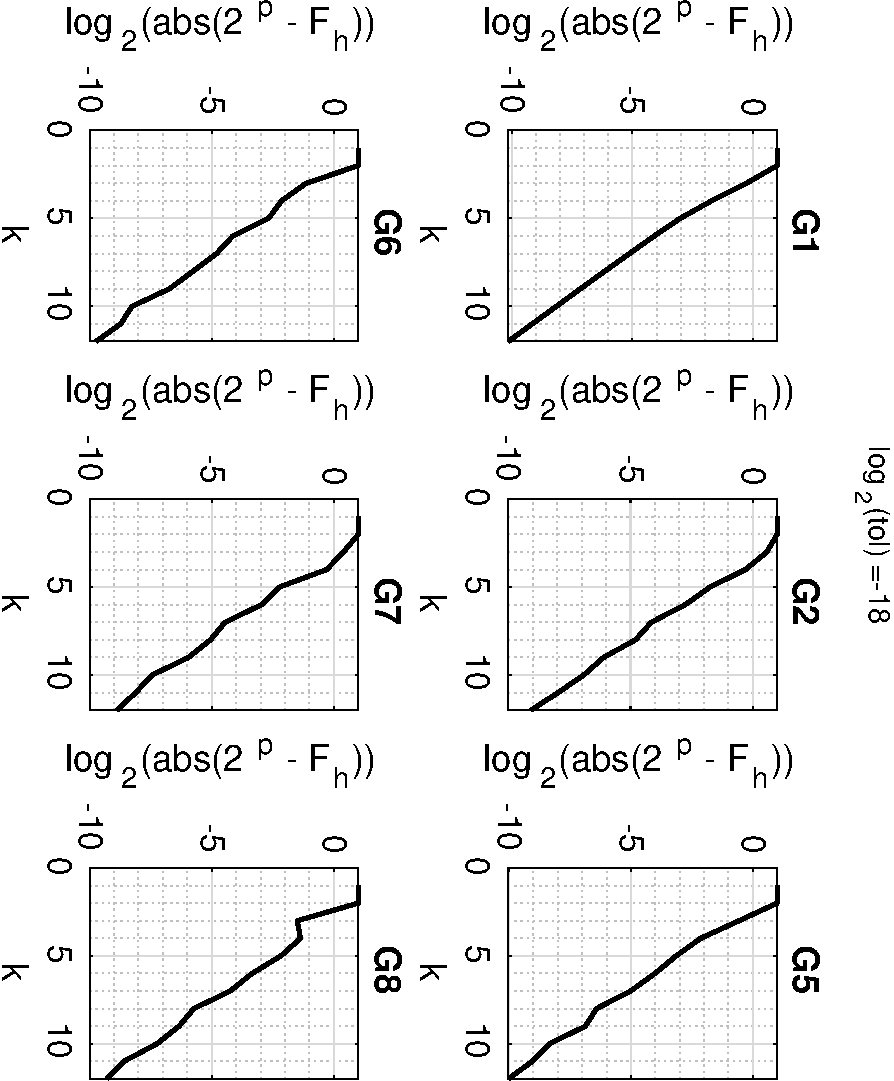
\includegraphics[width=10cm]{maxrange_rk1_tol18.pdf} \caption{The evolution of $F_h$ for 3 different drag coeffients, 1st order Runge-Kutta and sufficiently accurate event location.}
  \end{figure}

}


\frame{\frametitle{Computing the optimal range of the a howitzer: Failure}

 \begin{figure}
    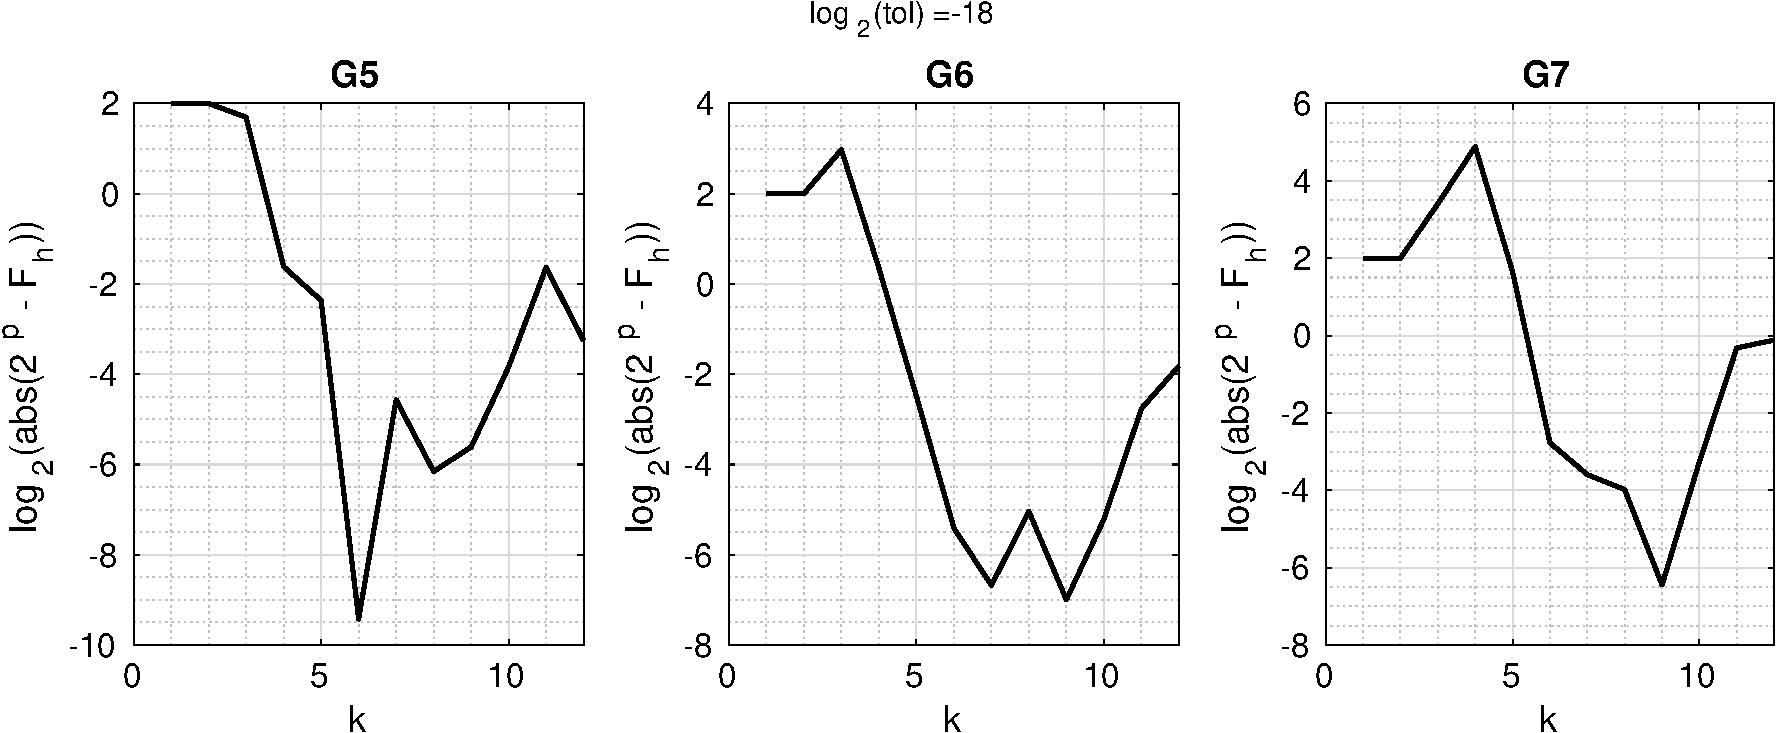
\includegraphics[width=10cm]{maxrange_rk2_tol18.pdf} \caption{The evolution of $F_h$ for 3 different drag coeffients, 2nd order Runge-Kutta and inaccurate event location.}
  \end{figure}
 
}


\frame{\frametitle{Modelling ions: Setup}

  The total force on an ion is given
  \begin{equation}
    \bm{F}(\bm{r_i}) =  - \alpha \sum_{j \not = i} \frac{1}{\|\bm{r}_i - \bm{r}_j\|^3}(\bm{r}_i - \bm{r}_j) - \beta \bm{r_i} - \gamma \bm{v}_i
  \end{equation}
  where $r_k$ is the position of the $k$th ion and $v_k$ is it velocity.
  \vspace{1cm}
  \begin{itemize}
  \item We wish to know the total kinetic energy $T$ at a fixed time.
  \item We compute approximation $A_{h_k}$ for $h_k = 2^{-k} h_0$.
  \end{itemize}
}

\frame{\frametitle{Modelling ions: Success}

   \begin{figure}
     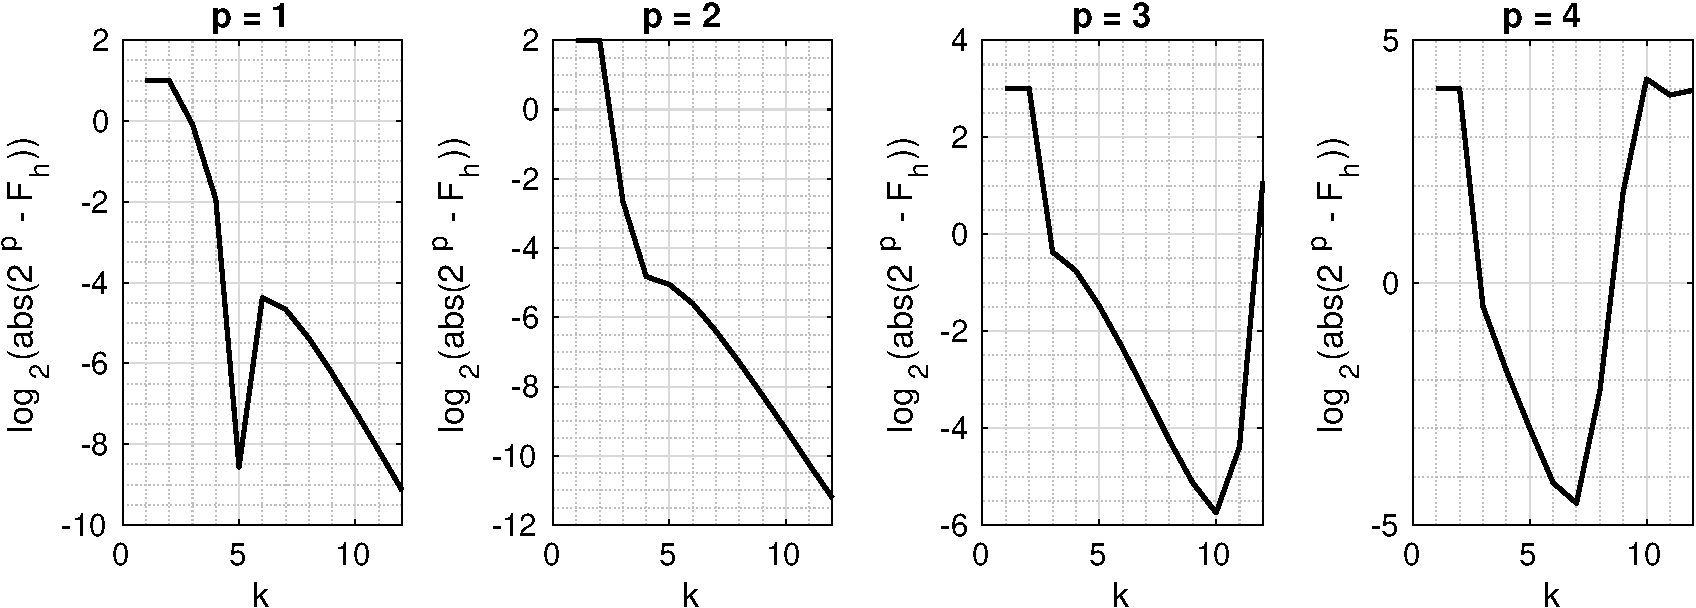
\includegraphics[width=10cm]{iontrap_mwe1.pdf}
     \caption{The evolution of $F_h$ for Runge-Kutta methods of order $p \in \{1,2,3,4\}$ and smooth force-fields with infinite range.}
  \end{figure}
}


\frame{\frametitle{Modelling ions: Failure}
 \begin{figure}
    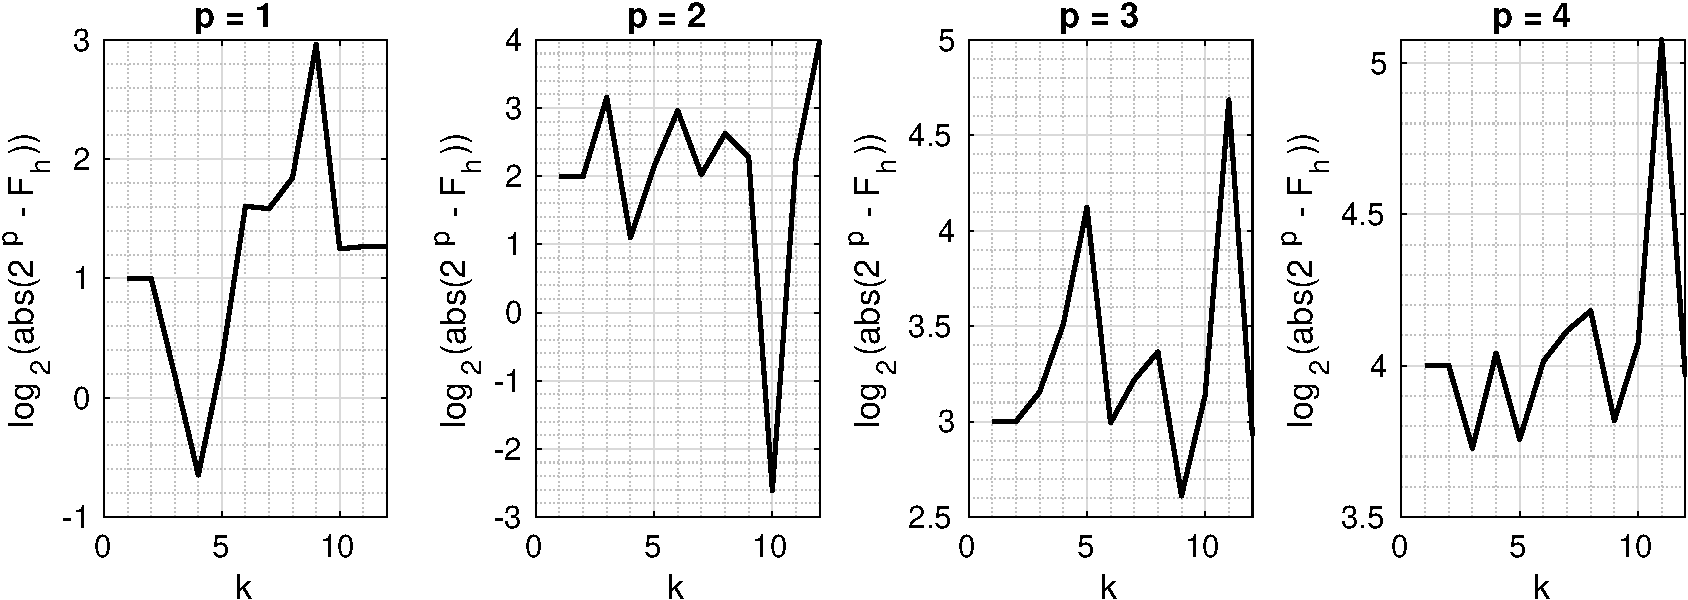
\includegraphics[width=10cm]{iontrap_mwe2.pdf} \caption{The evolution of $F_h$ for Runge-Kutta methods of order $p \in \{1,2,3,4\}$ and truncated force-fields with jump discontinuities.}
  \end{figure}
}

\frame{\frametitle{Modelling ions: Success}
 \begin{figure}
    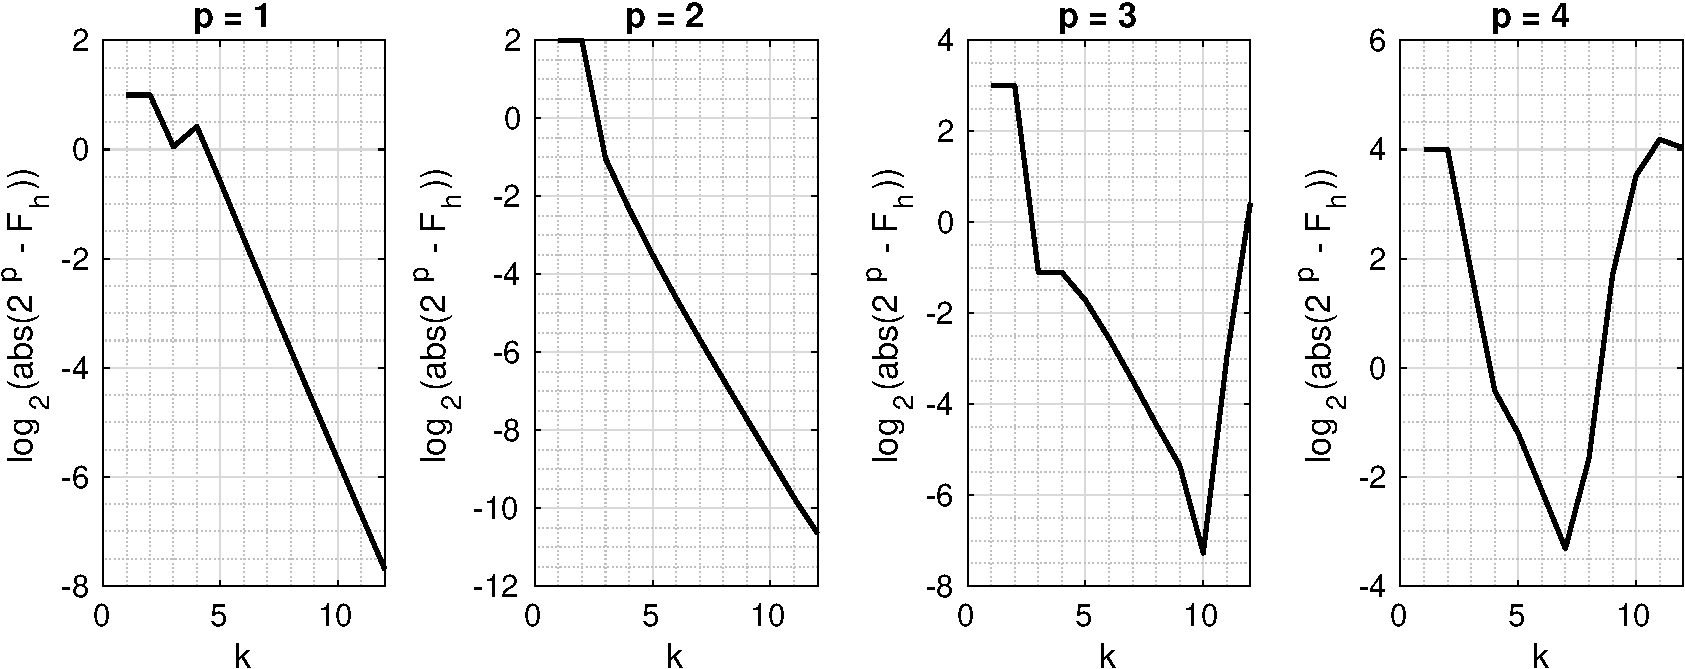
\includegraphics[width=10cm]{iontrap_mwe4.pdf} \caption{The evolution of $F_h$ for Runge-Kutta methods of order $p \in \{1,2,3,4\}$ and smoothly truncated force-fields.}
  \end{figure}
}





  
\frame{\frametitle{Why should this concern the computational scientist?}

  We use every trick in the book to
  \vspace{0.5cm}
  \begin{enumerate} \setlength\itemsep{1.5em}
  \item reduce time-to-solution
  \item increase the parallel efficicency
  \item reduce energy-to-solution
  \end{enumerate}
  \vspace{1cm}
  We should not forget to ask the question:
  \begin{center}
    \begin{large}
      \textbf{Can we still validate our models against the real world?}
    \end{large}
  \end{center}
}

\frame{\frametitle{Links}

  \begin{figure}
    
\includegraphics[width=6cm]{homepage.png}
  \end{figure}
  \begin{center}
    Thank your for your attention
  \end{center}
}

\end{document}
